\documentclass[10pt,a4paper,landscape]{article}
\usepackage[margin=15mm]{geometry}
\usepackage[T1]{fontenc}
\usepackage{libertinus}
\usepackage[scaled=0.93]{inconsolata}
\usepackage{microtype}
\usepackage{amsmath}
\usepackage{tikz}
\usetikzlibrary{arrows.meta,calc,positioning}
\usepackage{xcolor}
\pagestyle{empty}
\setlength{\parindent}{0pt}
\definecolor{ink}{HTML}{202A34}
\definecolor{secondary}{HTML}{5A6570}
\definecolor{linegray}{HTML}{A9B1B8}
\definecolor{lightgray}{HTML}{F6F7F8}
\definecolor{accent}{HTML}{31536E}
\tikzset{
  module/.style={rectangle, draw=linegray, line width=.65pt, fill=white,
    minimum height=2.18cm, minimum width=5.92cm, text width=5.40cm,
    align=left, inner xsep=3mm, inner ysep=2.5mm, anchor=north west},
  shared/.style={rectangle, draw=linegray, line width=.65pt, fill=lightgray,
    minimum height=1.62cm, minimum width=8.07cm, text width=7.51cm,
    align=left, inner xsep=3mm, inner ysep=2mm, anchor=north west},
  last/.style={rectangle, draw=accent, line width=.9pt, fill=white,
    minimum height=2.18cm, minimum width=5.92cm, text width=5.40cm,
    align=left, inner xsep=3mm, inner ysep=2.5mm, anchor=north west},
  arrow/.style={-{Stealth[length=2.3mm,width=1.5mm]},draw=accent,line width=.82pt},
  link/.style={draw=linegray,line width=.7pt},
  feedback/.style={draw=secondary,dashed,line width=.76pt,
    -{Stealth[length=2mm,width=1.3mm]}},
}
\newcommand{\head}[1]{{\sffamily\bfseries\color{ink}\fontsize{9.2}{10.5}\selectfont #1}}
\newcommand{\code}[1]{{\ttfamily\color{accent}\fontsize{8.2}{9.7}\selectfont #1}}
\newcommand{\bodyline}[1]{{\sffamily\color{secondary}\fontsize{8.2}{9.8}\selectfont #1}}
\begin{document}
\vspace*{-2.5mm}
{\sffamily\fontsize{13.8}{17}\selectfont\bfseries\color{ink}
Risk-aware, memory-augmented A2A market agents}\par
\vspace{1mm}
{\sffamily\fontsize{9}{11}\selectfont\color{secondary}
Week 08 midterm \;\textbar\; Student ID 25522018 \;\textbar\;
Implemented decision paths, bounded LLM harness, and verified settlement boundary}\par
\vspace{3.5mm}
\begin{center}
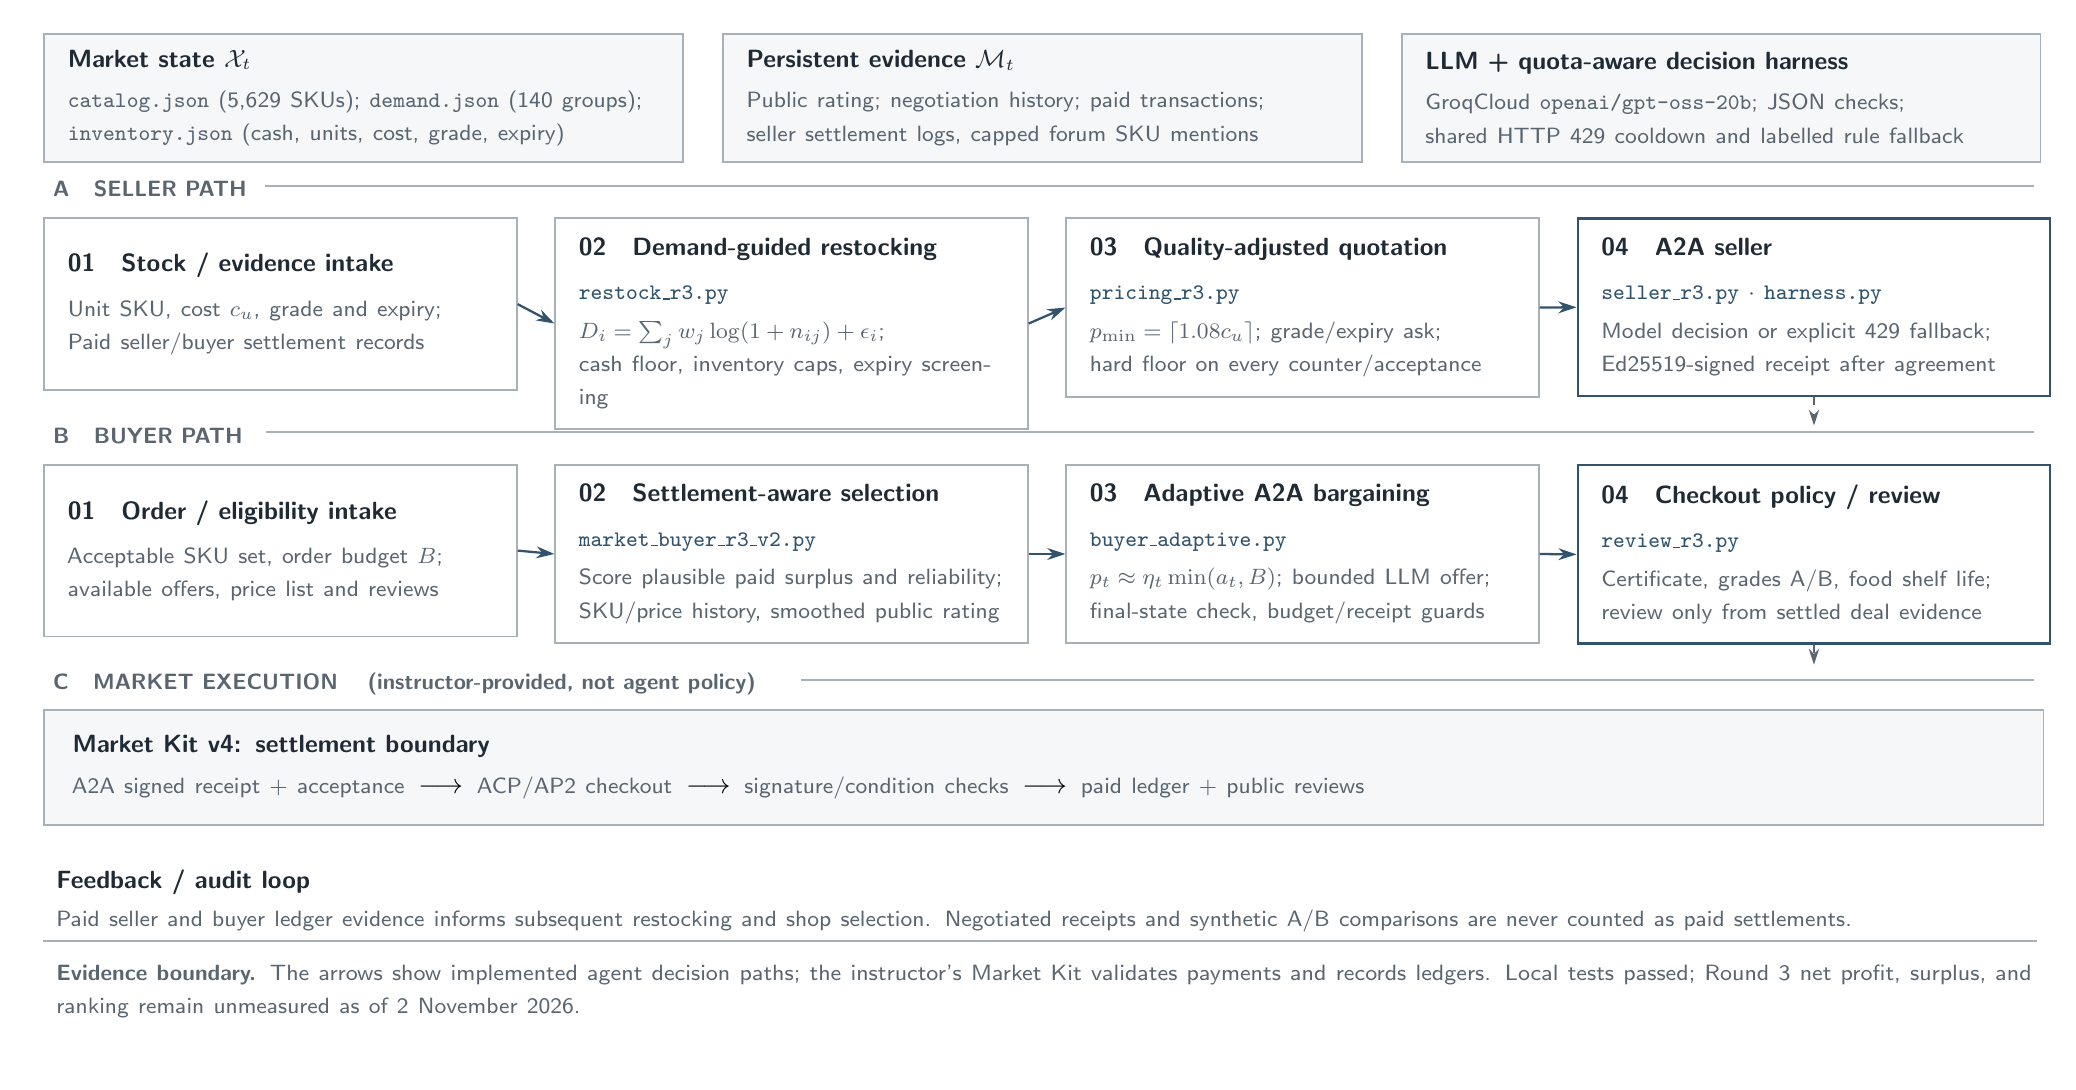
\begin{tikzpicture}[x=1cm,y=1cm]
\path[use as bounding box] (0,0) rectangle (25.65,13.13);

% 1. Thin source band: three shared services, no colored "dashboard" cards.
\node[shared] (source) at (0.20,13.06) {\head{Market state $\mathcal{X}_t$}\\[2.5pt] \bodyline{\texttt{catalog.json} (5,629 SKUs); \texttt{demand.json} (140 groups);}\\ \bodyline{\texttt{inventory.json} (cash, units, cost, grade, expiry)} };
\node[shared] (memory) at (8.82,13.06) {
  \head{Persistent evidence $\mathcal{M}_t$}\\[2.5pt]
  \bodyline{Public rating; negotiation history; paid transactions;}\\
  \bodyline{seller settlement logs, capped forum SKU mentions}
};
\node[shared] (model) at (17.44,13.06) {
  \head{LLM + quota-aware decision harness}\\[2.5pt]
  \bodyline{GroqCloud \texttt{openai/gpt-oss-20b}; JSON checks;}\\
  \bodyline{shared HTTP 429 cooldown and labelled rule fallback}
};

% Shared interface label in center.
\node[anchor=west,font=\sffamily\bfseries\fontsize{8.5}{10}\selectfont,text=secondary]
    at (.20,11.08) {A\quad SELLER PATH};
\draw[link] (3.02,11.12) -- (25.48,11.12);

% Seller row.
\node[module] (s1) at (.20,10.72) {
  \head{01 \; Stock / evidence intake}\\[4pt]
  \bodyline{Unit SKU, cost $c_u$, grade and expiry;}\\
  \bodyline{Paid seller/buyer settlement records}
};
\node[module] (s2) at (6.69,10.72) {
  \head{02 \; Demand-guided restocking}\\[4pt]
  \code{restock\_r3.py}\\[2pt]
  \bodyline{$D_i=\sum_j w_j\log(1+n_{ij})+\epsilon_i$;}\\
  \bodyline{cash floor, inventory caps, expiry screening}
};
\node[module] (s3) at (13.18,10.72) {
  \head{03 \; Quality-adjusted quotation}\\[4pt]
  \code{pricing\_r3.py}\\[2pt]
  \bodyline{$p_{\min}=\lceil1.08c_u\rceil$; grade/expiry ask;}\\
  \bodyline{hard floor on every counter/acceptance}
};
\node[last] (s4) at (19.67,10.72) {
  \head{04 \; A2A seller}\\[4pt]
  \code{seller\_r3.py $\cdot$ harness.py}\\[2pt]
  \bodyline{Model decision or explicit 429 fallback;}\\
  \bodyline{Ed25519-signed receipt after agreement}
};
\foreach \a/\b in {s1/s2,s2/s3,s3/s4}{\draw[arrow] (\a.east) -- (\b.west);}

% Middle text separates lanes with minimal marks.
\node[anchor=west,font=\sffamily\bfseries\fontsize{8.5}{10}\selectfont,text=secondary]
    at (.20,7.95) {B\quad BUYER PATH};
\draw[link] (3.03,7.99) -- (25.48,7.99);

% Buyer row
\node[module] (b1) at (.20,7.59) {
  \head{01 \; Order / eligibility intake}\\[4pt]
  \bodyline{Acceptable SKU set, order budget $B$;}\\
  \bodyline{available offers, price list and reviews}
};
\node[module] (b2) at (6.69,7.59) {
  \head{02 \; Settlement-aware selection}\\[4pt]
  \code{market\_buyer\_r3\_v2.py}\\[2pt]
  \bodyline{Score plausible paid surplus and reliability;}\\
  \bodyline{SKU/price history, smoothed public rating}
};
\node[module] (b3) at (13.18,7.59) {
  \head{03 \; Adaptive A2A bargaining}\\[4pt]
  \code{buyer\_adaptive.py}\\[2pt]
  \bodyline{$p_t\approx\eta_t\min(a_t,B)$; bounded LLM offer;}\\
  \bodyline{final-state check, budget/receipt guards}
};
\node[last] (b4) at (19.67,7.59) {
  \head{04 \; Checkout policy / review}\\[4pt]
  \code{review\_r3.py}\\[2pt]
  \bodyline{Certificate, grades A/B, food shelf life;}\\
  \bodyline{review only from settled deal evidence}
};
\foreach \a/\b in {b1/b2,b2/b3,b3/b4}{\draw[arrow] (\a.east) -- (\b.west);}

% Integration strip.
\node[anchor=west,font=\sffamily\bfseries\fontsize{8.5}{10}\selectfont,text=secondary]
    at (.20,4.80) {C\quad MARKET EXECUTION \;\; (instructor-provided, not agent policy)};
\draw[link] (9.82,4.84) -- (25.48,4.84);
\node[draw=linegray,fill=lightgray,line width=.65pt,anchor=north west,
      minimum width=25.39cm,minimum height=1.46cm,text width=24.67cm,align=left,
      inner xsep=3mm,inner ysep=2.5mm] (market) at (.20,4.48) {
  \head{Market Kit v4: settlement boundary}\\[3pt]
  \bodyline{A2A signed receipt + acceptance}\, $\longrightarrow$\,
  \bodyline{ACP/AP2 checkout}\, $\longrightarrow$\,
  \bodyline{signature/condition checks}\, $\longrightarrow$\,
  \bodyline{paid ledger + public reviews}
};
\draw[feedback] (s4.south) -- ++(0,-.36);
\draw[feedback] (b4.south) -- ++(0,-.25);

% Audit loop as a plain two-column footnote, not a giant decorative box.
\node[anchor=north west,align=left,text width=24.9cm] at (.24,2.56) {
  {\sffamily\bfseries\fontsize{8.8}{10.5}\selectfont\color{ink}Feedback / audit loop}\par\vspace{1.7pt}
  {\sffamily\color{secondary}\fontsize{8.5}{10.4}\selectfont
  Paid seller and buyer ledger evidence informs subsequent restocking and shop selection.
  Negotiated receipts and synthetic A/B comparisons are never counted as paid settlements.}
};
\draw[link] (.2,1.53) -- (25.52,1.53);
\node[anchor=north west,align=left,text width=25.1cm] at (.24,1.35) {
  {\sffamily\color{secondary}\fontsize{8.1}{10.3}\selectfont
  \textbf{Evidence boundary.} The arrows show implemented agent decision paths; the instructor's
  Market Kit validates payments and records ledgers. Local tests passed; Round 3 net profit,
  surplus, and ranking remain unmeasured as of 2 November 2026.}
};
\end{tikzpicture}
\end{center}
\vspace{-2.5mm}
{\sffamily\color{secondary}\fontsize{8}{10}\selectfont
\textbf{Figure 1.} Implemented Week 08 architecture. The GroqCloud model proposes actions;
code constrains prices and fallbacks. The instructor's Market Kit independently validates
ACP/AP2 settlement. The receipt binds \texttt{\{shop,item,price,task\}}.}
\end{document}
